% Created 2017-09-11 Mon 11:24
\documentclass[11pt]{article}
\usepackage[utf8]{inputenc}
\usepackage[T1]{fontenc}
\usepackage{fixltx2e}
\usepackage{graphicx}
\usepackage{longtable}
\usepackage{float}
\usepackage{wrapfig}
\usepackage{rotating}
\usepackage[normalem]{ulem}
\usepackage{amsmath}
\usepackage{textcomp}
\usepackage{marvosym}
\usepackage{wasysym}
\usepackage{amssymb}
\usepackage{hyperref}
\tolerance=1000
\usepackage[left=1in,right=1in,top=1in,bottom=1in]{geometry}
\usepackage{amsmath}
\date{September 11, 2017}
\title{Week 3 lecture notes - PSYC 5316}
\hypersetup{
  pdfkeywords={},
  pdfsubject={},
  pdfcreator={Emacs 25.2.1 (Org mode 8.2.10)}}
\begin{document}

\maketitle
In studies, our data amounts to a \emph{sample} of a population.  Based on our work in Week 2, we know that the \textbf{sample mean} $\overline{x}$ is the maximum likelihood estimator of the population mean $\mu$ (assuming a normal distribution as our model).  However, $\overline{x}$ is still an \textbf{estimate}, which means there is uncertainty in our measurement

Goal: develop a method that will give us a \textbf{range} of values for $\mu$ based on the available data $\overline{x}$

\section*{Sampling distributions}
\label{sec-1}

Definition: a \textbf{sampling distribution} for an estimator is the probability distribution for the values of that estimator.

Example: this week we will work exclusively with the sampling distribution for the \emph{sample mean}, denoted $\overline{X}$.
\begin{itemize}
\item Note: the notation can be confusing, so let's be very specific:
\begin{itemize}
\item $\overline{x}$ denotes the sample mean (an \emph{estimator})
\item $\overline{X}$ denotes the sampling \emph{distribution}
\end{itemize}
\end{itemize}


\subsection*{simulation of sampling distribution using R}
\label{sec-1-1}

We can simulate sampling distributions in R.  Below is some code that you can play with, but lets first understand the logic of the code.  For this simulation, lets assume our sample size is $n=25$.  Then, the basic loop is as follows:

\begin{enumerate}
\item take a sample of size 25 from the population.  Here, we'll assume that the population is normal with mean 50 and standard deviation 20.

\item compute the sample mean $\overline{x}$ of this sample
\item store the mean in a vector
\item do this a bunch of times (we'll do 5000 loops).
\end{enumerate}

Here is the code that accomplishes these steps:

\begin{verbatim}
N = 5000
Xbar=rep(0,N)
for (i in 1:N){
  Xsamp=rnorm(n=25, mean=50, sd=25)
  Xbar[i]=mean(Xsamp)
}
\end{verbatim}

Now, \texttt{Xbar} is a vector of 5000 sample means, which we can do all kinds of things with.  First, let's plot its density.  For comparison, we'll plot both the population density AND the sampling distribution together:

\begin{verbatim}
par(mfrow=c(2,1))
x=seq(-50,150,0.1)
plot(x,dnorm(x, mean=50, sd=25), type="l")
plot(density(Xbar),xlim=c(-50,150))
\end{verbatim}

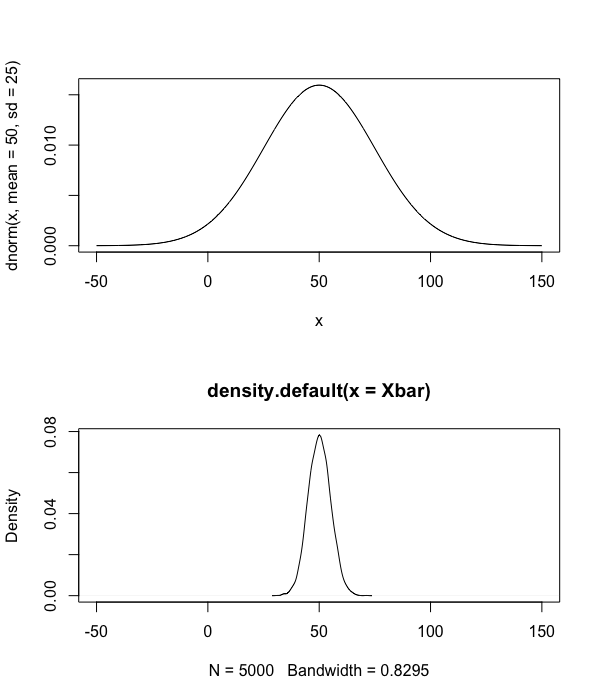
\includegraphics[width=.9\linewidth]{figures/week3/samp.png}

You might immediately notice a few things:
\begin{enumerate}
\item the sampling distribution appears normally distributed
\item the mean of the sampling distribution is equal to the mean of the population
\item the standard deviation of the sampling distribution is \textbf{much less} than the population standard deviation.
\end{enumerate}

We can check claims 2 and 3 easily:

\begin{verbatim}
mean(Xbar)
sd(Xbar)
\end{verbatim}

You should discover that the mean of $\overline{X}$ is also approximately equal to 50, and the standard deviation of $\overline{X}$ is approximately 5.  This is no accident, as is nicely summarized in the following:

Fact: when randomly sampling from a normal distribution, we have:
\begin{itemize}
\item the sampling distribution $\overline{X}$ is normal
\item $E(\overline{x})=\mu$
\item $\sigma_{\overline{X}} = \frac{\sigma}{\sqrt{n}}$, where $n$ = sample size
\end{itemize}

\subsection*{computing probabilities of samples}
\label{sec-1-2}

Consider an experiment that was designed to understand the effect of ozone on weight gain in rats. Suppose that weight gain in rats is normally distributed with $\mu=14$ and $\sigma=6$.

Suppose further that we test 22 randomly sampled rats.  We administer an ozone "treatment" to these rats and then subsequently measure their weight gain.  We find that $\overline{x}=11$.

Is it reasonable to expect a sample mean of $\overline{x}=11$ from the parent population?  Why/why not?

To solve this, think back to our work above.  Can we describe the distribution of sample means (assuming a sample size of $n=22$)?

\begin{itemize}
\item the sampling distribution $\overline{X}$ is normally distributed
\item $\mu_{\overline{X}}=22$
\item $\sigma_{\overline{X}} = \frac{\sigma}{\sqrt{n}} = \frac{6}{\sqrt{22}} = 1.279$
\end{itemize}

Based on this, we can use the \texttt{pnorm} function to compute the probability of obtaining a sample mean of 11 or less.

\begin{verbatim}
pnorm(11, mean=14, sd=1.279)
\end{verbatim}

We find that the probability of obtaining a sample mean of 11 or smaller is low.  Specifically, $p(\overline{x}\leq 11)=0.0095$.

\subsubsection*{Alternative: transform to $z$-scores}
\label{sec-1-2-1}
A more classical approach to this problem is to transform the raw data to a $z$-score.  Recall that if $X$ is normally distributed with mean $\mu$ and standard deviation $\sigma$, we can \textbf{standardize} $X$ via the transformation:

\[
Z=\frac{X-\mu}{\sigma}
\]

This \textbf{standard normal distribution} has mean 0 and standard deviation 1, and is the basis of all normal tables in the back of textbooks.

Another advantage of transforming to a $z$ score is that the \texttt{pnorm} computation is very easy!

In our example above (the rats), we could do the following:

\begin{enumerate}
\item convert the raw score $\overline{x}=11$ to a $z$-score:
\end{enumerate}

\[
z=\frac{\overline{x}-\mu_{\overline{X}}}{\sigma_{\overline{X}}}=\frac{\overline{x}-\mu}{\sigma/\sqrt{n}} = \frac{11-14}{6/\sqrt{22}} = -2.35
\]

\begin{enumerate}
\item compute $p(z\leq -2.345)$
\end{enumerate}

\begin{verbatim}
pnorm(-2.345)
\end{verbatim}


\section*{Confidence interval of population mean}
\label{sec-2}
For this section, we will assume that all parent distributions are normal.  We'll cover non-normality later.

\subsection*{Case 1: assume $\sigma$ is known}
\label{sec-2-1}
Recall from above that $Z=\frac{\overline{X}-\mu}{\sigma/\sqrt{x}}$ has a standard normal distribution.  Specifically, this gives us a few known facts about $Z$.  In particular:

\begin{itemize}
\item $p(-1.96 \leq Z \leq 1.96) = 0.95$
\end{itemize}

Note: you can verify this claim in R:

\begin{verbatim}
pnorm(1.96)-pnorm(-1.96)
\end{verbatim}

Let's work further with this.  If we substitute the expression for $Z$, we get 

\[
p\Biggl( -1.96 \leq \frac{\overline{X}-\mu}{\sigma/\sqrt{n}} \leq 1.96\Biggr) = 0.95
\]

We can rearrange terms in this inequality to express it in terms of $\mu$:

\[
p\Biggl( \overline{X}-1.96\frac{\sigma}{\sqrt{n}} \leq \mu \leq \overline{X}+1.96\frac{\sigma}{\sqrt{n}}\Biggr) = 0.95
\]

This is nice, because it says that even though we don't know the exact value of the population mean $\mu$, we know there is a 95\% probability that its value is between 

\[
\overline{X}-1.96\frac{\sigma}{\sqrt{n}}
\]

and 

\[
\overline{X}+1.96\frac{\sigma}{\sqrt{n}}
\]

This interval

\[
\Biggl(\overline{X}-1.96\frac{\sigma}{\sqrt{n}}, \overline{X}+1.96\frac{\sigma}{\sqrt{n}}\Biggr)
\]

is called the \textbf{95\% confidence interval} for $\mu$.  


Example: Suppose we obtained $\overline{x}=54$ from a sample of $n=25$.  Suppose further that we know that the population is normal, with unknown mean $\mu$, but known standard deviation $\sigma=9$.  Construct a 95\% confidence interval for the mean $\mu$.

From above, we compute

\[
\Biggl(54 - 1.96\frac{9}{\sqrt{25}}, 54 + 1.96\frac{9}{\sqrt{25}}\Biggr) = (50.5,57.5)
\]

Thus, we are 95\% confident that the population mean $\mu$ is between 50.5 and 57.5


\subsubsection*{General case:}
\label{sec-2-1-1}
There is nothing special about the quantity 95\%.  We can compute any confidence interval we wish!

Example: For 16 observations randomly sampled from a normal distribution, imagine that $\overline{X}=32$ and $\sigma =4$.  Construct a 90\% confidence interval for $\mu$.

To construct a 90\% interval, we must know the $z$ scores that contain 90\% of the standard normal distribution.  That is, we need to know the 0.05 quantile and the 0.95 quantile (this is because we need a total of 10\% combined in the upper and lower tails).

\begin{verbatim}
qnorm(0.05)
qnorm(0.95)
\end{verbatim}

We see that the two quantiles for the 90\% confidence interval are $\pm 1.645$.  Thus, we can compute:

\[
\Biggl(32 - 1.645\frac{4}{\sqrt{16}}, 32 + 1.645\frac{4}{\sqrt{16}}\Biggr) = (30.355, 33.645)
\]

Thus, we are 95\% confident that $\mu$ is between 30.355 and 33.645.


\subsection*{Case 2: assume $\sigma$ is NOT known}
\label{sec-2-2}

If $\sigma$ is NOT known, we will need an \emph{estimator} for it.

Recall that the definition of standard deviation is usually given as the square root of the variance, given by

\[
\frac{\sum (x-\mu)^2}{n}
\]

Unfortunately, this formula is well known to underestimate the actual value of the variance.  That is,

\[
E[\text{variance}] = \sigma^2 - \frac{\sigma^2}{n}
\]

However, if we adjust the formula for variance slightly to:

\[
s^2 = \frac{\sum (x-\mu)^2}{n-1}
\]

it can be shown that $E[s^2] = \sigma^2$.  That is, $s$ is an \emph{unbiased} estimate of $\sigma$.


\subsubsection*{Student's $T$ distribution}
\label{sec-2-2-1}

In 1908, William Gosset figured out how to quantify error when sampling from normal distributions from which the the standard deviation is \emph{unknown}.  He published his work using the psuedonym "Student"

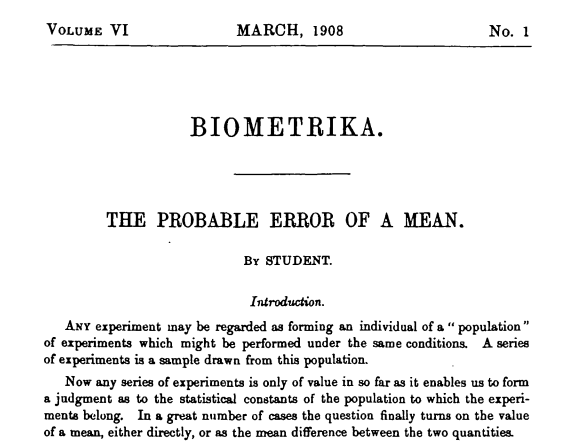
\includegraphics[width=.9\linewidth]{figures/week3/student.png}

Essentially, his method is based on computing something similar to the $z$ score.  Let

\[
T=\frac{\overline{X}-\mu}{s/\sqrt{n}}
\]

Notice that the only difference from $Z$ is that we have replaced $\sigma$ by the unbiased estimator $s$.

It turns out that the distribution $T$ is NOT a normal distribution; moreover, its shape depends on the sample size $n$.  Specifically, the parameter is \texttt{df} (degrees of freedom), where $df=n-1$.

Executing the following R commands will produce a nice plot demonstrating this:

\begin{verbatim}
dev.off()
x=seq(-3,3,0.01)
plot(x,dnorm(x),type="l")
lines(x,dt(x,df=5),lty=2)
lines(x,dt(x,df=20),lty=3)
legend(0,0.1,c("normal","df=5","df=20"),lty=1:3)
\end{verbatim}

As you can see in the figure, the T curves have heavier tails than the normal curve.  As 
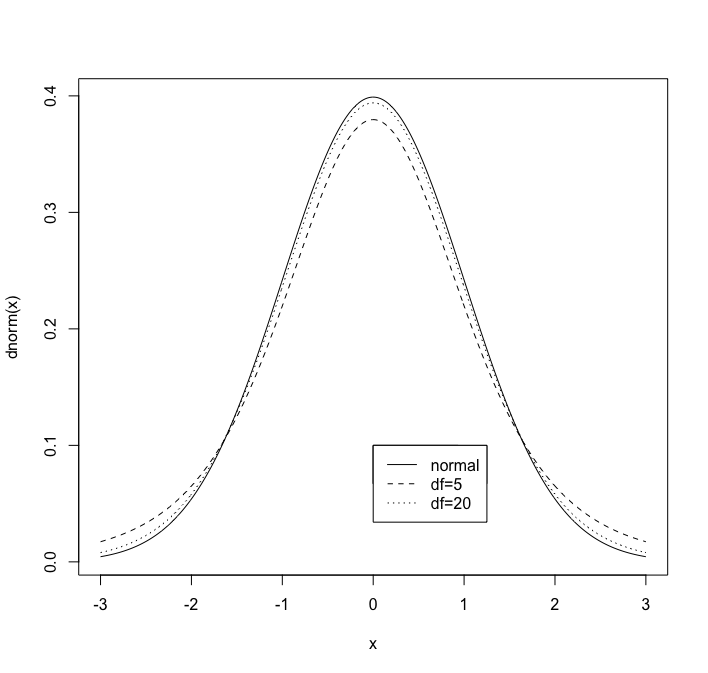
\includegraphics[width=.9\linewidth]{figures/week3/tDist.png}

\subsubsection*{Computing confidence intervals with with $T$}
\label{sec-2-2-2}

When $\sigma$ is not known, we can use the value of $s$ as an estimate for the population standard deviation. However, as we just saw, the resulting sampling distribution $T$ is not normal.  Thus, we can no longer use our old friend 1.96 to compute a 95\% confidence interval.  We have to compute confidence intervals using different bounds.

Example:  Lets go back to our rats from above.  We tested 22 rats and got a sample mean of $\overline{x}=11$.  Assume further that our sample standard deviation is $s=19$.  Compute a 90\% confidence interval for the population mean $\mu$.

Similar to before, we will compute the interval

\[
\Biggl(\overline{X}-c\cdot \frac{s}{\sqrt{n}}, \overline{X}+c\cdot \frac{s}{\sqrt{n}}\Biggr)
\]

To find $c$, we need to know the 0.05 and 0.95 quantiles of the $T$ distribution on 21 degrees of freedom.

\begin{verbatim}
qt(0.05, df=21)
qt(0.95, df=21)
\end{verbatim}

Thus, we see that our interval is:

\[
\Biggl(11-1.72\cdot \frac{19}{\sqrt{22}}, 11+1.72\cdot \frac{19}{\sqrt{22}}\Biggr) = (4.03, 17.97)
\]

Example:  Suppose we test a new reading instruction method on 4th graders and obtain the following scores on a reading test: 

12, 20, 34, 45, 34, 36, 37, 50, 11, 32, 29

Suppose further that the \emph{standard} methods of reading instructions produce an average score on this test of 25.  Does the new reading method increase reading scores?

To answer this, we will compute a 95\% confidence interval for $\mu$, the population of reading scores under this NEW method:

\begin{verbatim}
read=c(12,20,34,45,34,36,37,50,11,32,29)

length(read) # easy way to compute sample size

Xbar=mean(read)
s=sd(read)

c=qt(0.975,df=10) # compute 0.975 quantile

Xbar-c*s/sqrt(10) # lower limit
Xbar+c*s/sqrt(10) # upper limit
\end{verbatim}

We can see that our 95\% confidence interval is (22.2,39.6).  Since this interval contains 25, we are not confident that the new reading method increases reading scores.


\section*{What happens when sampling from non-normal distribution?}
\label{sec-3}
\subsection*{Central limit theorem - if $n$ is large enough, $Z$ has standard normal distribution}
\label{sec-3-1}
\begin{itemize}
\item how large must $n$ be?
\item demonstrate using R some sampling distributions from:
\begin{itemize}
\item uniform
\item exponential
\end{itemize}
\end{itemize}

\subsection*{demonstrate how $t$ is susceptible to influence}
\label{sec-3-2}
Recall that confidence intervals based on $t$ scores assume normality.  How \emph{robust} is the $t$ distribution to violations of this assumption?

\begin{itemize}
\item Case 1: heavy tailed distributions
\end{itemize}

Let's simulate a \emph{contaminated normal} distribution.  This is a distribution where scores come from two different underlying normal distributions: one

\begin{itemize}
\item lognormal
\item lognormal + heavy tails
\end{itemize}
% Emacs 25.2.1 (Org mode 8.2.10)
\end{document}